Pred se lahko izdela primerjavo podatkovnih struktur je potrebno predstaviti okolje, v katerem bo izdelana primerjava, metoda uporabljena za izdelavo primerov ter testni primeri, ki so uporableni za izdelavo primerjve.

\subsection{Stroj, operaciski sistem in metoda testiranja}
Za izdelavo primerjva podatkovnih struktur bo uporabljen računalnik s procecorjem Intel Core i3 5005U z dvema jedroma in štirimi nitmi ter s taktom $1,9$ GHz. Računalnikima na razpolago 4 GB delovnega pomnilnika, od katerega je ob zagonu zasedengea $1,35$ GB z operaciskim sistemom ter emulatorejm terminala (angl. \textit{terminal emulator}). Poleg delovnega pomnilnika ima računalnik še $8$ GB Swap razdelka na trdem disku, ki je namenjen shranjevanju neuporabljenih pomnilniških strani v primeru prezasedenega delovnega pomnilnika in posledično sproščanju le tega. Operaciski sistem računalnika je Fedora 42 in uporabljen Linux kernel je 6.14.11-300.

Za vsako primerjano podatkovno strukturo bodo izmerjene tri strari: prostor, ki ga zasede na pomnilniku, čas potreben za izgradnjo podatkovne strukture ter čas potreben za izvršitev poizvedb v podatkoni strukturi. Struktura primerjava je prikazana s psevdokodo na Algoritmu \ref{alg:metodaTest}. Vsak test v primerjavi se izvede 5-krat, da se zmanjša vpliv drugih procesov na rezultate tetiranja. Iz psevdo kode opazimo, da primerjva poizved bo storjena za poizvedbo $\Prisotnost{T}{P}$, saj je pogosto vprašanje v biologiji prisotnost gena (vzorcev) v DNK sekvenci (vhodna beseda), ne pa natančen položaj tega gena ali števila ponovitev gena v DNK sekvenci. Poizvedba je bila izdelana za vzorce velikosti 5, 50, 500 in $\log{|T|}$ (na psevdokodi $\log{i}$). Rezultati testiranja so shranjeni v CSV datoteko in vsaka vrstica datoteke, shrani sledeče podatke: podatkovna struktura, velikost vhodne besede, čas izgradnje, čas iskanja vzorca dolžine 5, čas iskanja vzorca dolžine 50, čas iskanja vzorca dolžine 500, čas iskanja vzorca dolžine $\log{|T|}$ ter velikost podatkovne strukture. Velikost bo dodana ročno iz podatkov priboljenih s pomnilniškim profilerjem (angl. \textit{memory profiler}). 

\begin{algorithm}[htb]

\Vhod{Vhodno beseda $T$, število znakov v najdaljšem testiranem nizu $i_{max}$}
\Izhod{CSV datoteka z izračunanimi časi}
\caption{Psevdokoda primerjave indeksov}\label{alg:metodaTest}
{
    {$i \leftarrow 500$}
    
    \Dokler{$i \le i_{max}$}{

        \Za{$S\in\{ST, SA, SA+LCP, CST\}$}{
            \Za{$k=1\dots 5$}{
                {$\textit{start}\leftarrow \textit{čas}()$}

                {$\textit{Izgradi}(S,T[1:i-1]\cdot\$)$}

                {$\textit{konec}\leftarrow \textit{čas}()$}

                {$t_{Izg}\leftarrow \textit{konec} - \textit{start}$}

                \Dokler{$j \le 500$}{
                    {$\textit{start}\leftarrow \textit{čas}()$}

                    {$\Prisotnost{S}{T[i:i+j]}$}

                    {$\textit{konec}\leftarrow \textit{čas}()$}

                    {$j\leftarrow j*10$}

                    {$t_{j} \leftarrow \textit{konec} - \textit{start}$}
                }

                {$j\leftarrow \log{i}$}

                {$\textit{start}\leftarrow \textit{čas}()$}

                {$\Prisotnost{S}{T[i:i+j]}$}

                {$\textit{konec}\leftarrow \textit{čas}()$}

                

                {$t_{log} \leftarrow \textit{konec} - \textit{start}$}

                {$\textit{Shrani}(S,i,t_{Izg},t_{5},t_{50},t_{500},t_{log}$)}

                {$\textit{Izbriši}(S)$}
            }
        }        
        
        {$i \leftarrow i+500$}
        
    } 
    
}
\end{algorithm}


Primerjava podatkovnih struktur je izdelana v programskem jeziku C++\footnote{Koda je dostopna na povezavi \url{https://github.com/GioGiou/MagisterskaNalogaKoda}.}. Zato se čase potrebne za izgradnjo struktur ter poizvedb v njih izmeri z beleženjem trenutnega časa pred začetkom, ki ga shranimo v spremenljivko \verb|start|, in po koncu operacije, ki pa ga shranimo v spremenljivko \verb|stop|. Meriteve so implementirane s funkcijo \verb|high_resolution_clock::now()|, ki je del standardne knjižnice programskega jezika C++ in vrne natančen čas trenutka, v katerem jefunkcija izvedena. Čas izvajanja se lahko naračuna kot razlika med časom ob koncu izvajanja in časom ob začetku izvajanja operacije, kar se v C++ stori s funkcijo \verb|duration_cast<nanoseconds>(stop - start)| \verb|.count()|. Za izgradnjo podatkovnih struktur bodo uporabljeni sledeče knjižnice. Priponsko drevo uporabila implementacijo iz knjižnice \cite{ganeshk13}, ki implemenira Ukkonenov algoritem \cite{Ukkonen1995}. Kompaktna priponska drevesa so bila izdelana s implementacijo iz knjižnice SDSL \cite{gbmp2014sea}. Priponska polja pa so bila implementira s pomočjo knjižnice \cite{Grebnov2025}, ki izgradi priposnko polje v $O(n)$ časa z algorimom, ki sta ga predstavila Timoshevskaya in Feng \cite{Timoshevskaya2014}. Algoritem je izboljšava predhodno predstavljenga aligoritma od Ko in Aluru \cite{Ko2005}. Podatkovna struktura LCP polje, ki je bila predstavljena v podpoglavju \ref{sec:SAPoizvedbe} in sicer podatkovna struktura $Q-LCP$, izračunana v času $O(n)$. Knjižnica \cite{Grebnov2025} sicer podpira izgradnjo LCP strukture, ki je bila predstavljena v podpoglavju \ref{sec:STsimulacija}, ampak nima dodatne podatkovne strukture Fischer-Heun za operacijo $rmq$ v konstantnem času \cite{Fischer2007}.

Poleg časovne zahtevnosti izgradnje in pozved v podatkovnih strukturah nas zanima, koliko prostora posaminčna podatkovna struktura zasede na delovnem pomnilniku. In sicer nas zanima največji zaseden prostor v času izgradnje posamične podatkovne strukture. Le ta bo izmerjen z uporabo pomnilniškega profilerja. Uporabljen bo pomnilniški profiler Bytehound \cite{Bytehound2024}, saj omogoča grafični prikaz porabe pomnilnika v času izvajanja programa.

Ker je primerjava izdelana v C++, je potrebno kodo prevesti v izvršljivo datoteko. To je strojeno s prevajalinkom GCC 15.1.1. Program je bil preveden s sledečim ukazom:
\begin{lstlisting}[language=bash]
    g++ -std=c++11 -O3 -DNDEBUG -I ./include -L ./lib // 
    main.cpp -o main -lsdsl -ldivsufsort //
    -ldivsufsort64 -lsuffix -lsais
\end{lstlisting}
\newpage
Pri prevajanju programa je uporabljenih nekaj zastavic, ki določajo vrednosti parametrov prevajalnika. Večina zastavic je vezana na uvažanje knjižnic v prevajanje, in sicer \verb|-I ./include| nastavi pot do zaglavnih datotek (angl. \textit{header files}), \verb|-L ./lib| nastavi pot do strojne kode knjižnice ter zastavice \verb|-lsdsl|, \verb|-ldivsufsort|, \verb|-ldivsufsort64|,  \verb|-lsais| in \verb|-lsuffix| uvozijo potrebne knjižnice za izgradnjo izvršljive datoteke.
Zastavica \verb|-O3| določa nivo optimizacije izvršljive datoteke, na nivo 3, ki je bil izbran, saj je uporabljen za prevajanje prve implementacije kompaktnega priponskega drevesa \cite{Valimaki2007}. Ker se uporablja profiler, je potrebo pred začetkom testiranja indeksov besed zagnati tudi profiler, kar je storjeno z ukazom:
\begin{lstlisting}[language=bash]
    export MEMORY_PROFILER_LOG=info
    LD_PRELOAD=~/bytehound/libbytehound.so ./main // 
    ./test/NaKlancu.txt 
\end{lstlisting}
Prva vrstica ukaza določa stopnjo profiliranja, ki ima v tem primeru vrednost \verb|info|, ter se jo shrani v sistemsko spremenljivko \verb|MEMORY_PROFILER_LOG|. Naslednja vrstica pa požene program ter se poda kot prvi parameter ime datoteke s testnimi podatki. Zgornji ukaz prikaže primer za vhodno besedilo Na klancu. S spremenljivko \verb|LD_PRELOAD| je določen deljeni objekt (angl. \textit{shared object}), ki je izvršen pred začetkom programa. V primeru testiranja je deljeni objekt profiler, kar mu omogoča dostop do programa in lažje beleženje zasedenega delovnega spomina.

Dolžina najdaljše vhodne besed $i_{max}$ je bila sprva nastavljena na 4000000 znakov. Med testiranjem priponskega drevesa besede dložine 2048000 znakov se je opazilo, da čas potreben za izgradnjo prvega priponskega drevesa presega 5 minut. Po petih minutah od začetka izgradnje drevesa lahko poazimo, da je delovni pomnilnik skoraj v celoti zaseden ter je Swap razdelek zaseden že z 6 GB pomnilniški strani. Pri tem je računalnik  neodziven in proces je v neprekinjenem spanju (angl. \textit{Uninterruptible sleep} ali stanje D). Na Sliki \ref{fig:6GB} je prikazan upravljalnik opravil Htop v času izgradnje priponskega drevesa za besedo dolžine 2048000 znakov. Proces v modri vrstici predstavlja program za testiranje čas izgradnje in pozvedb ter postorske zahtevnosti indeksov besed. V stolpcu označenim S (Stanje ali angl. \textit{Status}) je vidno, da je je stanje procesa označeno kot D, ker je proces v neprekinjenem spanju. Po več kot 5 minutah od začetka izgradnje priponskega drevesa za besedo dolžine 2048000 znakov sem se odločil, da se proces ubije. Posledično se je znižala velikost besede za izgradnjo zadnjega indeksa na 1024000 znakov. Med testiranjem sem opazil tudi, da se $LCP$ polje ne izgradi za besede dolžine 1024000 znakov, zato sem se odločil, da se ta test v tem koraku izpusi.

\begin{figure}[tb]
    \centering
    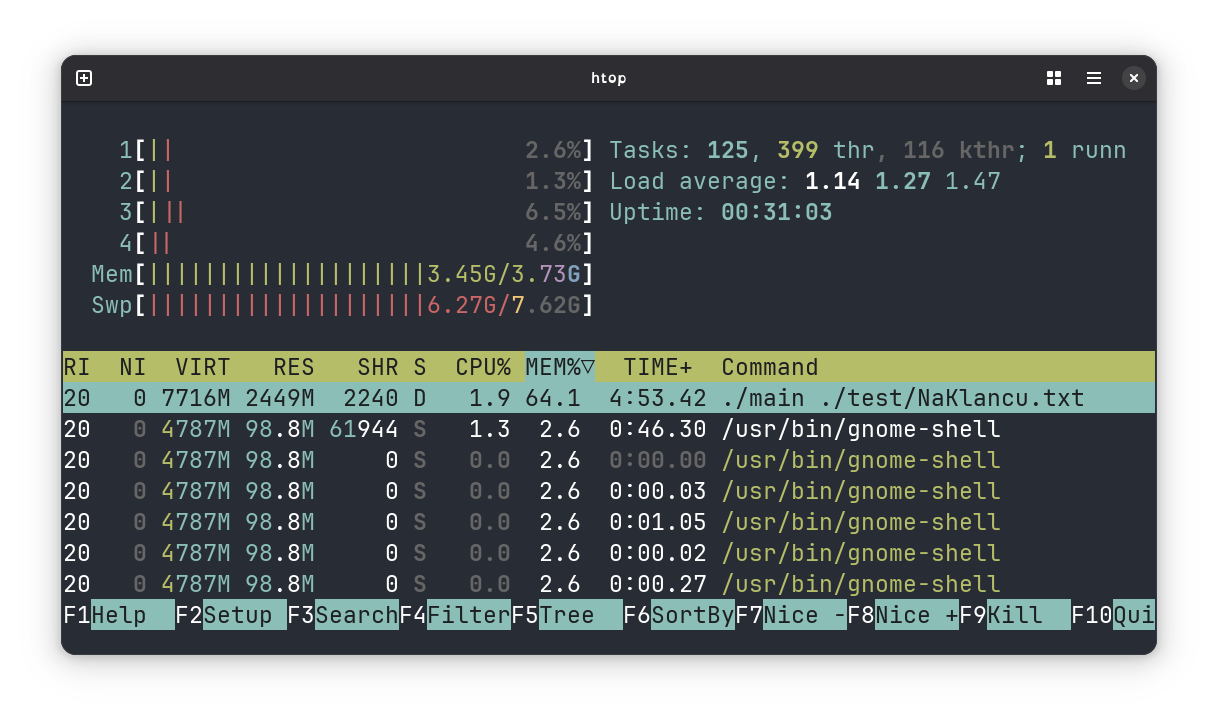
\includegraphics[width=\textwidth]{Slike/Zaslonski posnetek 2025-06-23 22-53-56.png}

    \captionof{figure}[Posnetek zaslona upravljalnika opravil Htop med izgradnjo priponskega drevesa za besedilo dolžine 2048000 znakov.]{Posnetek zaslona upravljalnika opravil Htop med izgradnjo priponskega drevesa za besedilo dolžine 2048000 znakov.} 
    \label{fig:6GB}
\end{figure}
\newpage

\subsection{Testni primeri}

Predstavljeno tesno metodo bomo pognali nad dvemi vhodnimi besedili prikazanih v Tabeli \ref{tab:besedila}. Prva testirana beseda je Cankarjev kratki roman Na klancu \cite{podatkiNaKlancu}. Roman je bil izbran, saj predstavlja tipično vhodno besedo naravnega jezik, ki je v tem primeru slovenščina. Abeceda takih besed sestoji iz črk naravenga jezika (velikih in malih), presledkov in ločil. Pri tem se je pojavil probelm, saj slovenščina ne uporablja ASCII znake. Zato je potrebno pred samim začetkom testiranja vhodno besedo pred pripraviti. To je bilo storjeno tako, da so bili vsi ne ASCII znaki odstranjeni oziroma zamenjani z ASCII alternativami. Na primer znak, ki predstavlja '...', je bil zamenjan s tremi pikami, vse črke z naglasi (kot so strešice, ostrivci ter drugi) so bile zamenjani z osnovnim znakom, torej na primer š postane s in é postane e. Pri tem so bile tudi odstranjene vse prazne vrstice ter ločila poglavij, ki so bila označena z '***'. Odstranjeni so bili tudi vsi nevidni simboli, ki niso videni bralcu, prisotni v besedilu. Na ta način se je začetno besedilo znižalo iz dolžine 319843 znakov na 317803 znakov pred podaljševanjem.

\begin{table}[htb]
    \caption{Primerjava besedil, ki bodo uporabljena za primerjavo različnih implementacij priponskih dreves}
    \label{tab:besedila}
    \centering
    \begin{tabular}{rccc}
        Ime testne besede& Število znakov & Velikost abecede & Velikost na disku \\
        &  &   & [MB]\\
         \hline
        Ivan Cankar, Na klancu \cite{podatkiNaKlancu}& 317803 & 52 & $25,851$ \\
        DNK sekvenca \cite{podatki}&  52428800& 4 & $26,767$ \\
    \end{tabular}    
\end{table}

Druga testirana beseda pa je daljša DNK sekvenca \cite{podatki}, ki je zlepek različnih DNK sekvenc. Izbrana je bilam kot primer vhodne besede uporabljene v bioinformatiki. Ta vhodna beseda je bila predhodno uporabljena za testiranje implementacije kompaktnega priponskega drevesa od Välimäki idr. \cite{Valimaki2007}

\paragraph{Podalševanje besedila.}

V drugem stolpcu Tabele \ref{tab:besedila} so prikazane dolžine besed, ki bodo uporabljen za testiranje. Pri tem se opazi, da nekatera besedila so krajša kot 2048500 znako, ki so potreni za izgradnjo indeksov in za izdelavo vzorcev testiranja. Zato je treba te besede podalšati. Ker je malo verjetno, da se vhodno besedilo ponovi $k$-krat, dokler ne doseže primerne velikosti, predvsem v naravnem jeziku, bo uporabljena bolj napredna metoda podaljševanja besedila. Metoda vzame manjše podnize besedila ter naredi stik med začetno besedo in podnizom. Tako dobljeno besedilo je bolj verjetno, saj je večja verjetnost, da se manjši deli besedila ponovijo za razliko od celotnega besedila. Predlagana metoda podaljševanja besedila je prikazana na Algoritmu \ref{alg:Konkatenacija}. Pri tem metoda predpostavi, da je besedilo dolgo vsaj $3000$ znakov. Ta metoda je primerna za podaljševanje daljših besedil, sicer pa je možno metodi spremeniti parameter $i$ in tako prilagoditi metodo drugim besedilom.


\begin{algorithm}[htb]

\Vhod{Vhodno besedilo $T$, želena velikost $s_{max}$}
\Izhod{Besedilo $T_0$}
\caption{Metoda podaljševanja vhodnega besedila}\label{alg:Konkatenacija}
{
    {$T_0\leftarrow T$}

    {$i\leftarrow 500$}
    
    \While{$|T_0| < s_{max}$}{
        
        {$T_0\leftarrow T_0\cdot T[i:6i]$}
        
        
        {$i\leftarrow i+500$}

        \While{$6i>|T|$}{$i=i/4$}
        
    }
    \Vrni{$T_0[1:s_{max}]$}    
    
}
\end{algorithm}

Predlagana metoda podaljša besedo na velikost $s_{max}$. Ta velikost je lahko dolžina najdaljšega besede ali pa je poljubna vrednost, bodisi manjša od največjega besede bodisi večja. Če je beseda daljša od velikosti $s_{max}<|T|$, bo predlagana metoda skrajšala besedo na $|T_0|=s_{max}$. Za potrebe testiranja sem se odločil, da je $s_{max}=25000000$, kar je več kot zadostna dolžina.


%V tem poglavju je opisana empirična primerjava časovnih zahtevnosti različnih operacij, poizvedb in izgradnje ter prostorske zahtevnosti različnih implementacij priponskega drevesa. Priponsko drevo se uporablja za iskanje vzorcev v besedilu $T$, torej se je smiselno osredotočiti zgolj na primerjavo časovnih zahtevnosti za poizvedbe ter za izgradnjo priponskega drevesa. Primerjava posamičnih operacij priponskega drevesa nima smisla, saj se le te uporabljajo pri implementaciji poizvedb in izgradnji. 
%
%Pri tem se bomo osredotočili zgolj na osnovne poizvedbe. Kot najbolj preprosta osnovna operacija bo izdelana primerjava nad poizvedbo $prisotnos(vzorec)$. Ta poizvedba je bila izbrana, saj je pogosto vprašanje v biologiji prisotnost genov (vzorcev) v DNK sekvenci, ne pa natančen položaj tega gena ali števila ponovitev vzorca. Čas izvajanja poizvedbe bo izmerjen kot razlika v času takoj pred začetkom izvajanja poizvedbe ter takoj po zaključku izvajanja poizvedbe. Poizvedba bo izmerjena na vzorcih dolžine 5 znakov, 50 znakov, 500 znakov in $\log{n}$ znakov, kjer je $n$ dolžina znaka. 
%
%Na podoben način kot poizvedba $prisotnos(vzorec)$ bo izmerjen tudi čas izgradnje priponskega drevesa. Le ta bo izmerjen s pomočjo razlike v uri med časom ure takoj pred izgradnjo ter v časom ure takoj po izgradnji priponskega drevesa.
%
%Izmerjeni časi bodo shranjeni v vektorju potrebnih časov $T_{i,v}$, pri čemer $i$ predstavlja dolžino vhodnega besedila in $v$ predstavlja tip priponskega drevesa (priponsko drevo z vrednostjo $v=ST$ ali kompaktno priponsko drevo z vrednostjo $v=CST$). Vektor bo sestavljen na sledeči način
%\begin{equation*}
%    T_{i,v}=(t_{izg},t_5,t_{50},t_{500},t_{\log{n}}),
%\end{equation*}
%pri čemer so izmerjeni časi za poizvedbe izmerjeni v nanosekundah, čas izgradnje $t_{izg}$ pa v milisekundah. 
%
%Na podoben način bo shranjena tudi velikost, ki jo zasede priponsko drevo v delovnem spominu. Izmerjen prostor bo poleg prostora priponskega drevesa vseboval tudi besedilo $B_{0}$, katerega podniz $B_0[1,i]$ bo uporabljen za izgradnjo. Ker bodo vse meritve vsebovale velikost besedila $B_0$, le to ne bo vplivalo na primerjavo podatkov. Izmerjen prostor bo shranjen v vektorju $S_{i,v}$, pri čemer $i$ predstavlja dolžino vhodnega besedila in $v$ predstavlja tip priponskega drevesa (priponsko drevo z vrednostjo $v=ST$ ali kompaktno priponsko drevo z vrednostjo $v=CST$). V tem primeru bo vektor $S_{i,v}$ vseboval zgolj vrednost $s_{max}$, ki je največja dosežena velikost priponskega drevesa med izvajanjem izgradnje in poizvedbe. Največji izmerjeni zasedeni prostor na delovnem spominu bo izmerjen z uporabo pomnilniškega profilerja (angl. \textit{memory profiler}).
%
%Uporabljeni bo Bytehound \cite{Bytehound2024} pomnilniški profiler, saj omogoča grafični prikaz porabe spomina v času izvajanja programa. Primer prikaza porabe delovnega spomina v času izvajanja testa je prikazan na Sliki \ref{fig:ZasedonestRAM}. Na sliki se jasno vidi, da večanje priponskega drevesa povzroči rast zasedenega prostor na delovnem spominu v času izgradnje in poizvedbe. Na sliki se lahko opazi, da izgradnja in poizvedbe v kompaktnem priponskem drevesu potrebujejo krepko manj časa in prostora, zato izgleda, kot da se graf konča malo pred koncem vodoravne osi. Razlog za to je izgradnja in poizvedba nad kompaktnim priponskim drevesom, ki potrebuje manj pomnilnika in posledično manj časa za dodeliti in sprostiti delovni spomin.
%
%\begin{figure}[tb]
%    \begin{center}
%        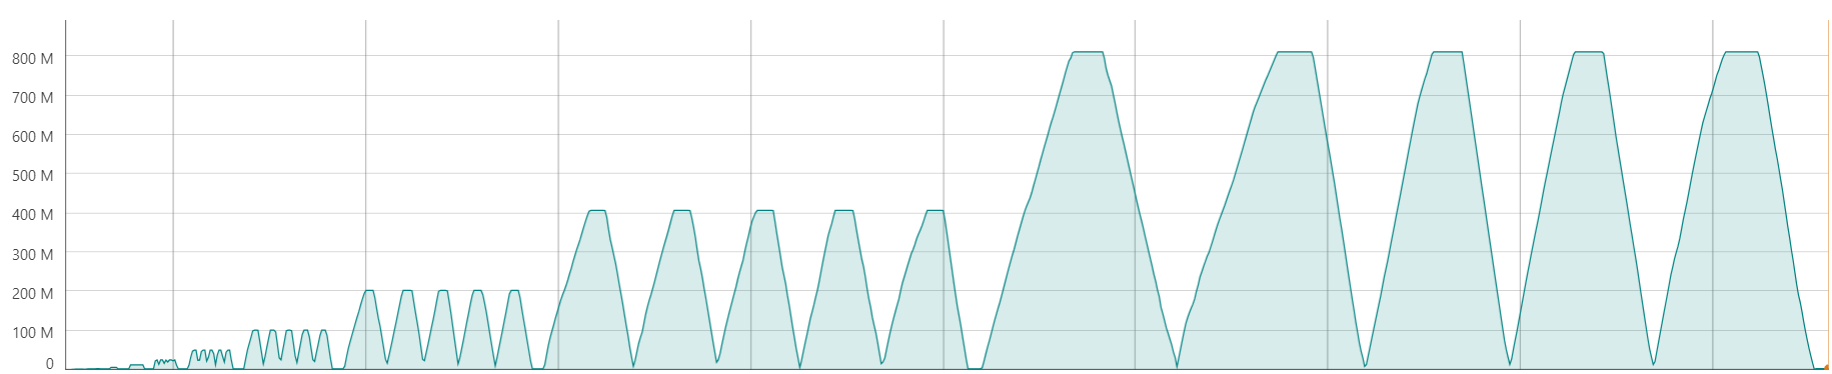
\includegraphics[width=\textwidth]{Slike/bytehoundGraf.png}    
%        \captionof{figure}[Zasedenost spomina testiranjem različnih implementacij priponskega drevesa skozi celotno izvajanje testa.]{Zasedenost spomina testiranjem različnih implementacij priponskega drevesa skozi celotno izvajanje testa.} 
%        \label{fig:ZasedonestRAM}    
%    \end{center}
%\end{figure}

%
%Za zmanjšati vpliv ostalih procesov na računalniku, se je vsak test ponovil 5-krat. To je tudi vidno na Sliki \ref{fig:ZasedonestRAM}, zato ima zadnje izgrajeno prionsko drevo 5 vrhov in vsak vrh predstavlja eno ponovitev testiranja. S pomočjo profilerja je bila tudi izmerjena velikost originalnega besedila $B_0$, ki je prikazan v zadnjem stolpcu Tabele \ref{tab:besedila}, saj se velikost razlikuje glede na vhodno besedilo.
%

%
%S tem načinom testiranja se želita ugotoviti dve stvari. Najprej se želi ugotoviti vpliv velikosti vhodnega besedila na čas izgradnje in poizvedb nad priponskim drevesom ter velikost spomina, ki ga zasede priponsko drevo. To bo izmerjeno z izgradnjo različnih dreves ter s poizvedbami nad njimi. Prvo drevo bo izgrajeno nad besedilom dolžine 500 znakov. Vsako naslednje priponsko drevo bo izgrajeno nad besedilom, ki je dvakrat daljše od predhodnega. Zadnje izgrajeno priponsko drevo bo imelo dolžino besedila, za katerega je bilo izgrajeno, manjšo od $|B_0|-500$ znakov ali $|B_0|-\log{(500\cdot2^{i-1})}$ za besedila daljša od $2^{500}$ znakov. V besedilu mora bit vedno na voljo dovolj znakov, da se bodo lahko iz njih naredili vzorci vseh testiranih velikosti. Besedilo, ki bo uporabljeno za izgradnjo $i$-tega priponskega drevesa, bo podniz $B_0[1,500\cdot2^{i-1}]$.
%
% Druga stvar, ki se želi ugotoviti, je vpliv uporabe \verb|swap| razdelka za namene delovnega spomina ter vpliv velikosti abecede vhodnega besedila in vzorca na iskanje vzorca v priponskem drevesu. Zato bo primerjava narejena na dveh besedilih, ki imata različno vhodno abecedo, in sicer prvo vhodno besedilo je kratki roman Ivana Cankarja, Na klancu \cite{podatkiNaKlancu}, ki uporablja slovensko abecedo, ter daljša DNK sekvenca \cite{podatki}, ki pa uporablja abecedo $\Sigma = \{A,C,T,G\}$. Pri tem obe abecedi ne vsebujeta znaka, ki predstavlja konec besedila, $\$$, saj bo le ta dodan besedilu pred začetkom izgradnje. Več podatkov o vhodnih besedilih je prikazanih na Tabeli \ref{tab:besedila}.
%
%
%\subsection{Pred obdelava besedil}
%
%Kot je razvidno v drugem stolpcu Tabele \ref{tab:besedila} je potrebno najkrajše besedilo podaljšati. Ker je malo verjetno, da se vhodno besedilo ponovi $k$-krat, dokler ne doseže primerne velikosti, predvsem v naravnem jeziku, bo uporabljena bolj napredna metoda podaljševanja besedila. Metoda vzame manjše dele besedila dolžine $5i$ ter jih konkatenira na koncu besedila. Tako dobljeno besedilo je bolj verjetno, saj je večja verjetnost, da se manjši deli besedila ponovijo za razliko od celotnega besedila. Predlagana metoda podaljševanja besedila je prikazana z Algoritmom \ref{alg:Konkatenacija}. Pri tem metoda predpostavi, da je besedilo dolgo vsaj $6i$, kar je $3000$ znakov dolgo. Ta metoda je primerna za podaljševanje daljših besedil, sicer pa je možno metodi spremeniti parameter $i$ in tako prilagoditi metodo drugim besedilom.
%

%
%%\newpage
%\subsection{Iskanje vzorcev}
%
%Po izgradnji priponskega drevesa bo le to uporabljeno za iskanje vzorcev v besedilu. Kot je bilo predhodno omenjeno, se bo pregledovala zgolj prisotnost vzorca v besedilu. Velikosti vzorcev, ki bodo iskani v besedilu so 5, 50 in 500 znakov ter $\lfloor\log{(500\cdot2^{i-1})}\rfloor$ znakov, pri čemer je $i$ zaporedna številka testa velikosti priponskega drevesa. Vzorec dolžine $x$ ($x$ je ena od predhodno naštetih velikosti vzorca) je pridobljen kot $B_0[500\cdot2^{i-1}+1,500\cdot2^{i-1}+1+x]$. 
%
%Vzorci, ki so izdelani na tak način, zagotavljajo, da z visoko verjetnostjo niso prisotni v besedilu ter posledično niti v priponskem drevesu. To naredi test bolj realističen, saj ko vemo, da je vzorec prisoten v besedilu, nima smisla preverjati pristnost vzorca. Če pa je besedilo $B_0$ podaljšano, na kakršen koli način, je prisotnost vzorca v besedilu večja.